\documentclass[class=report, crop=false, 12pt,a4paper]{standalone}
\usepackage{enumitem}
\usepackage{float}
\usepackage[normalem]{ulem}
\usepackage{graphicx}
\usepackage{amsmath}
\usepackage{siunitx}
\usepackage{commath}
\usepackage{tikz}
\usetikzlibrary{positioning, fit, calc}   
\tikzset{block/.style={draw, thick, text width=3cm ,minimum height=1.3cm, align=center},   
line/.style={-latex}     
}  
\begin{document}
\section{Fluid Machines}
Fluid machines are devices that operate by exchanging energy with a fluid. Fluid is a phase of matter unable to support a shear stress in static equilibrium. Fluids do not resist to deformation and take the shape of the containers (they flow). Fluids are also divided into liquids and gases. \textbf{Pumps} add energy to the fluid, resulting in an increase in fluid pressure across the machine. \textbf{Turbines} extract energy from the fluid, resulting in a decrease in fluid pressure across the machine.

Fluid machines are classified on the basis of the movement producing the energy transfer.
\begin{itemize}
  \item \textbf{Reciprocating machines} - energy is supplied or extracted by the reciprocating motion of a plunger or piston
  \item \textbf{Turbomachines} - energy is supplied or extracted by a rotating shaft
\end{itemize}
Fluid machines can also be classified on the basis of the way of treating the volume of fluid.
\begin{itemize}
  \item \textbf{Positive-displacement machines} - energy is supplied or extracted to/from a closed volume of fluid
  \item \textbf{Dynamic machines} - energy is supplied or extracted to/from an open volume (usually through rotating blades)
\end{itemize}
Taking into account of both classifications, pumps can be divided into three main categories:
\begin{itemize}
  \item \textbf{Reciprocating positive-displacement machines} - energy is supplied or extracted by the reciprocating motion of a piston acting on the boundaries of a closed volume of a fluid
  \item \textbf{Positive-displacement rotary machines} - energy is supplied or extracted by the movement of rotating components acting on a closed volume of fluid
  \item \textbf{Roto-dynamic machines} - energy is supplied or extracted to an open volume by the movement of rotating blades
\end{itemize}
\subsubsection*{Positive-displacement reciprocation pumps}
Positive-displacement pumps supply energy to the fluid by the movement of the boundaries of a closed volume: Fluid is sucked into an expanding volume and then pushed along as that volume contracts, producing an increase in fluid pressure.

For example, in a reciprocating positive displacement piston pump, the piston moves backwards, reducing the fluid pressure in the cylinder. The pressure decrease causes an inlet check valve to open, so that the fluid is sucked through the inlet check valve into the expanding volume. Then the piston moves forward, pushing the fluid volume and the increasing the fluid pressure. The pressurised liquid closes the inlet valve and lifts an outlet valve, leaving the chamber at higher pressure. Energy is supplied by the reciprocating motion of a piston acting on a closed volume of fluid.

Technical characteristics
\begin{itemize}
  \item Capacity - is low and discontinuous (pulsatile)
  \item Net head - high (even at low speeds)
  \item Efficiency - independent of capacity and head and good for any liquid
  \item Adjustment of capacity - obtainable by sending back part of outlet flow to the inlet
  \item Treatable liquids - viscous, hot and chemically aggressive and shear sensitive
  \item Self-priming - when dry can generate negative pressures that lift the liquid to the pump
  \item Starting torque - high and similar to the working torque
  \item Flow continuity - flow is discontinuous and needs a damping volume for smoothing
  \item Obstruction - can generates unacceptable high outlet pressures (safety valves required)
  \item Dimensions - relatively large, heavy and expensive
\end{itemize}
\subsubsection*{Positive-displacement rotary pumps}
Positive displacement pumps supply energy to the fluid by the movement of the boundaries of a closed volume. Fluid is sucked into an expanding volume and then pushed along as that volume contracts, producing an increase in fluid pressure.

Lobe, gear and screw rotary pumps: volumes of fluid are trapped in the pockets between the lobes (or the gear tooth spaces) and the casing. With the rotation of the loves (or gears) the liquid is forced to travel in one direction around the interior of the casing and is pushed through the outlet port under pressure. Lobes are driven by external timing gears and as a result the lobes do not make contact. Liquid travels around the interior of the casing in the pockets between the lobes and the casing, meshing of the lobes forces liquid through the outlet port under pressure. Energy is supplied by the movement of rotating components acting on a closed volume of fluid. 

Technical characteristics
\begin{itemize}
  \item Capacity - depends on the shaft speed
  \item Net head - high (even at low speeds) and independent from of shaft speed
  \item Efficiency - depends on the internal tolerance and their change during use
  \item Flow continuity - flow is uniform and continuous
  \item Do not need valves - the closed volume is trapped by the rotating components
  \item Dimensions - compact, light and relatively cheap
  \item Starting torque - high and similar to the working required torque
  \item Treatable liquids - viscous but free from sand, fibres or impurities
  \item Adjustment of capacity - requires change of operating speed (not always possible)
\end{itemize}
\subsubsection*{Positive-displacement peristaltic pumps}
Positive-displacement pumps supply energy to the fluid by the movement of the boundaries of a closed volume. Fluid is sucked into an expanding volume and then pushed along as that volume contracts, producing an increase in fluid pressure.

Peristaltic pumps: It is based on the principle of "peristalsis" (alternating contraction and relaxation of muscles around a tube). A smooth wall flexible tube is squeezed along its length, positively displacing the fluid contained within the tube. The tube's restitution after the squeeze creates a vacuum, which sucks more fluid into the tube, causing a gentle pumping action with minimal damage to the media inside the tube.
\subsubsection*{Roto-dynamic pumps}
Dynamic pumps supply energy to an open volume of fluid. In the case of roto-dynamic pumps, this is done by imparting to the flowing fluid a momentum through the rotation of the blades (impeller blades or rotor blades). (There are also non rotary dynamic pumps such as jet pumps or electromagnetic pumps.) The rotating blades are called \textbf{impeller blades} (or \textbf{rotor blades}) in the case of pumps. If the blades have a casing around the turbomachine it is called \textbf{enclosed} or \textbf{ducted}. If there is no casing, it is called \textbf{open}. 

Axial flow pumps: pressure is developed by the propelling or lifting action of the blades of the impeller on the liquid. These act as rotating wings, and produce force through application of both Bernoulli's principle and Newton's third law, generating a difference in pressure the forward and rear surfaces of the airfoil-shaped blades. Axial pumps give much lower pressures than centrifugal pumps.

Radial flow pumps: radial flow pumps are centrifugal pumps in which the pressure is developed wholly by centrifugal force: the fluid enters the pump near the centre of the impeller and is moved to its outside diameter by the rotating motion of the impeller. This allows centrifugal pumps to produce continuous flows at high pressure. 

Mixed flow pump: are intermediate between the previous two cases. The pressure is developed partly by centrifugal force and partly by the lift of the vanes of the impeller on the liquid. 

Technical characteristics
\begin{itemize}
  \item Capacity - increases with the operating speed and reduces with the fluid viscosity
  \item Net head - increases with the operating speed$^2$ and reduces with the fluid viscosity
  \item Efficiency - depends on the capacity and head and decreases with the fluid viscosity
  \item Required torque - depends on the operating speed
  \item Starting torque - ver low, compared to the operating torque
  \item Dimensions - compact light and economic
  \item Operating devices - electro-motors or turbo-motors can be used
  \item Flow continuity - flow is steady
  \item Tolerances - are not critical
  \item Adjustment of capacity - affects the efficiency
  \item Treatable fluids - they are not suitable for viscous fluids and shear sensitive fluids
\end{itemize}
\subsubsection*{Positive-displacement pumps}
Advantages
\begin{itemize}
  \item They are less traumatic for the fluid - are ideal to handle with shear sensitive fluids such as those in the food industry or blood (all pumping devices in animals are positive-displacement pumps)
  \item If well sealed, they are self-priming pumps - they can create a vacuum pressure at their inlet, even when dry (empty of liquid), sufficient to lift a liquid for several meters below the pump
  \item They run at relatively low speed - they need much less speed than dynamic pumps to operate at similar loads (fatigue and wearing are more reduced)
\end{itemize}
Disadvantages
\begin{itemize}
  \item Their volume flow rate does not change unless operating velocity is changed - usually it is not simple because AC electric motors are designed to operate at one or more fixed speeds
  \item If obstructed, they can create very high pressure at the outlet side - this may overload the driving motors, that may fail (overpressure protection is required)
  \item They may deliver a discontinuous flow (pulsatile) - this may be unacceptable for some applications
\end{itemize}
\subsubsection*{Dynamic pumps}
Advantages
\begin{itemize}
  \item They are mechanically simple - because of their simplicity, they are relatively economic and low maintenance
  \item Tolerances are not critical - since they are momentum based, they operate with a large range of mechanical tolerances. For the same reason, they are suitable for low viscosity fluids. 
  \item Provide a steady flow at the outlet - contrary to many positive displacement pumps
\end{itemize}
Disadvantages
\begin{itemize}
  \item They are not suitable for highly viscous fluids - due to the large amount of work required to rotate the impellers in this case
  \item They produce high levels of shear on the fluid - they should not be used to pump shear sensitive fluids (such as blood)
  \item They are not self-priming pumps - if empty, they do not create vacuum pressure sufficient to rise fluids for meters
\end{itemize}
\begin{figure}[H]
  \centering
  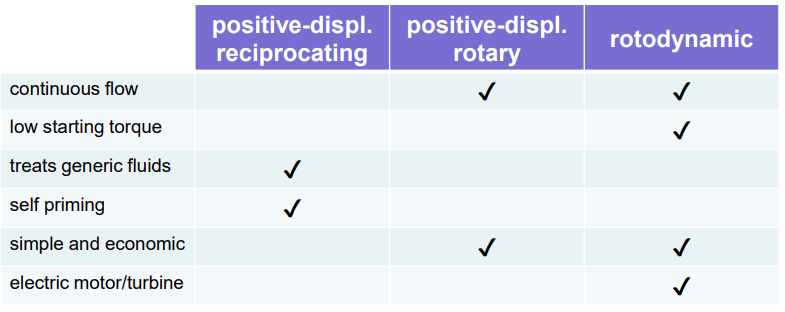
\includegraphics[width = 0.8 \textwidth]{../img/tabletocomparepumps.png}
\end{figure}
\end{document}